\section{\label{sec:electronicMatter}Band Theory and The Hall experiment}

\subsection*{\label{ssec:free-electron}Band Theory}

In the free electron model of a metal, non-interacting electrons form an electron gas and freely move around the solid and fill up energy levels while obeying the exclusion principle \cite{kittel_introduction_2004}. At $T = 0\ K$, the highest-filled energy level is the Fermi Energy, $E_F$. With the potential energy $V(r) = 0$, the electron wave function is a solution to the time-independent Schrodinger equation: 
\begin{align}
    -\dfrac{\hbar^{2}}{2m_e}\nabla^{2}\ket*{\phi(k)} = E\ket*{\phi(k)} \\
    \text{with } \ket*{\phi(k)} = A e^{i k r} \\
    \text{and energy eigenvalues } E = \dfrac{\hbar^{2}k^{2}}{2m_e}
    \label{eq:3dHamiltonian}
\end{align}

\begin{figure}[thpb] %this figure will be at the right
    \centering
    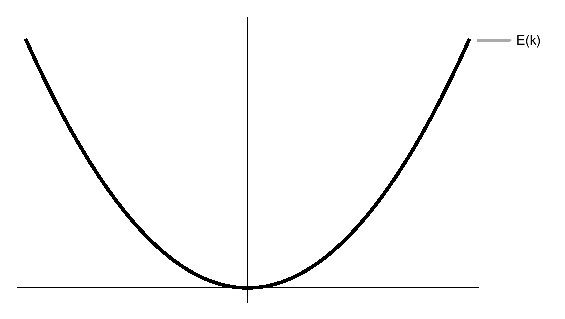
\includegraphics[width=0.25\textwidth]{figs/ek-free.eps}
    \caption{\label{fig:ek-free}Free electron dispersion relation.}
\end{figure}

The free electron model assumes a constant potential in the solid, as well as a impenetrable barrier at the edges of the solid. Modeling electrons in a solid as being in a periodic potential rather than completely free provides a better understanding of material properties (e.g insulator, metal, semimetal, semiconductor). Here, the potential drops at each lattice points where  ion cores (sources of the potential) are located, with the periodicity of the inter-atomic separation $a$. Due to the interaction between electrons (fermions) and the exclusion principle, degeneracy is split for the large number ($N$) of electrons in the lattice's periodic potential, which forms energy bands. Given the symmetry of the periodic potential ($U(r + na) = U(r)$), solutions to the Schrodinger equation are limited to so-called Bloch wavefunctions. Using \textbf{Bloch's Theorem} to represent the  wavefunctions, we have:

\begin{align}
    \ket{\Psi_{\mb{k}}(\mb{r})} = u_{\mb{k}}(\mb{r})e^{i\mb{k.r}} \\
    \text{with } u_{\mb{k}}(\mb{r} + n\mb{a}) = u_{\mb{k}}(\mb{r}) 
\end{align}

\begin{figure}[thpb]
    \centering
    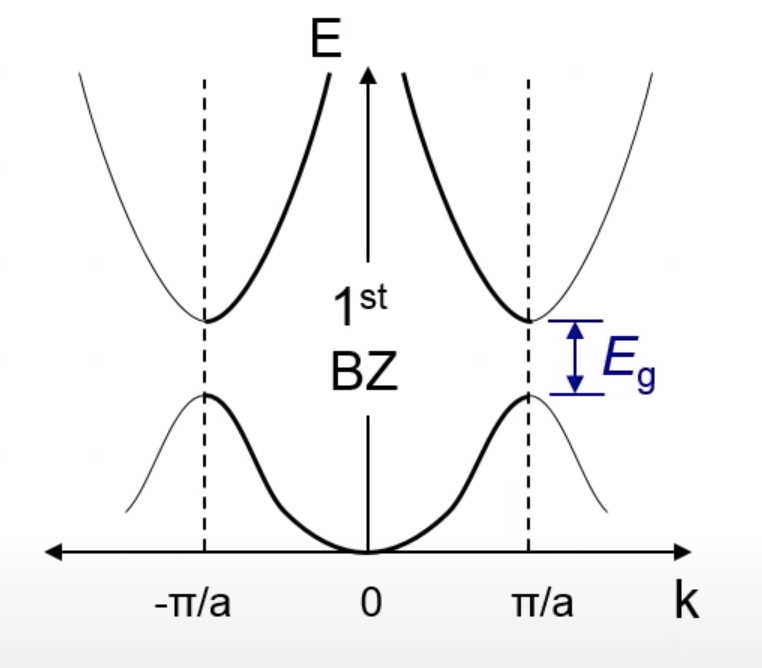
\includegraphics[width=0.25\textwidth]{figs/nfe-ek.png}
    \caption{\label{fig:ek-nfe}Reduced Zone Disperson Relation of an Electron in a Periodic Potential}
    \end{figure}

The dispersion relation in the reduced first Brillouin Zone (BZ) shows the expected energy bands, with band gaps due to Bragg diffraction of the electron waves at the edges of the BZ. The energy gap ($E_{g}$) reveals a \textit{forbidden zone} that cannot be occupied by the electrons' energy levels. Depending on where $E_{F}$ lies for the system and the number of electrons per atom, bands can be half-filled (metal), or filled (insulators). \textcolor{red}{This gap is already indicating different states of matter, and a phase transition...}

\subsection*{\label{ssec:classic-hall}The Classical Hall experiment}
In an experiment in 1879, Edwin Hall discovered that when a 2D conductor with current passing through it is placed in a strong magnetic field perpendicular to the plane of the electrons motion, the moving charges experience a Lorentz force ($F \propto j_{x}, B_{z}$) which pushes carriers on one side of the conductor, deflecting $j_{x}$). The concentration of charges of different signs on two edges of the conductor establishes an electric field which, in steady state, balances the Lorentz force. The from the electric field emerges a potential proportional to the current $j_{x}$ and the magnetic $B_{z}$ field, and perpendicular to both. 

\begin{figure}[thpb]
    \centering
    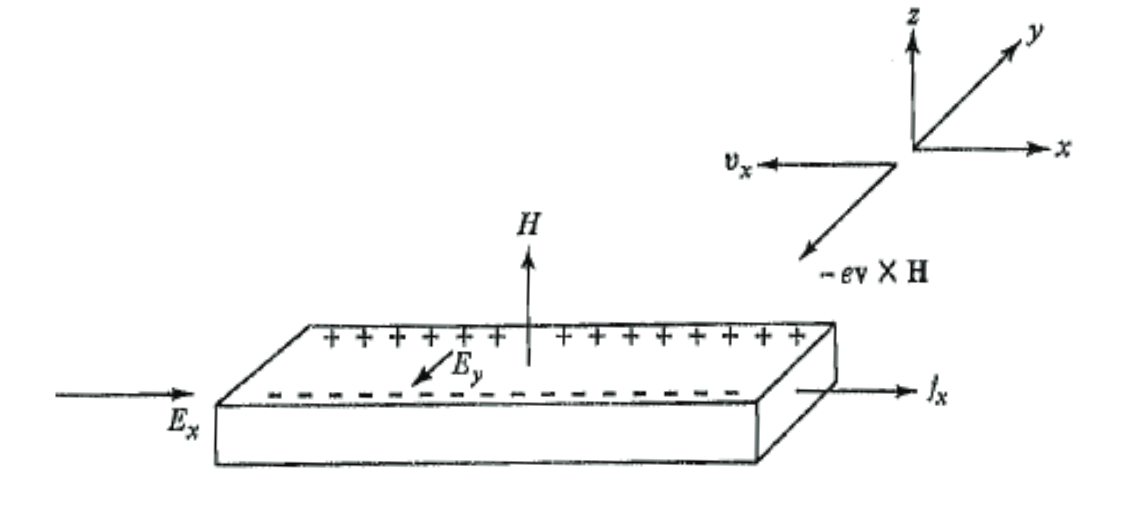
\includegraphics[width=0.25\textwidth]{figs/Hall.png}
    \caption{\label{fig:hall}Hall Experiment}
    \end{figure}

    From the Hall experiment it is possible to leverage the Drude model of metals and derive the following quantities that are relevant for the study of phases of matter based on topological invariants.

\begin{align}
    & \text{\textbullet\ Lorentz\ Force: } \mb{F} = q \mb{v} \times \mb{B} \\
    & \text{\textbullet\ Equilibrium\ condition: } j_{y} = 0 \\
    & \text{\textbullet\ Magnetoresistivity: }  \rho_{xx} = \dfrac{E_{x}}{j_{x}} \\
    & \text{\textbullet\ Hall (off-diagonal) resistivity: } \rho_{yx} = \dfrac{E_{y}}{j_x} \\
    & \text{\textbullet\ Hall coefficient: } R_{H} \equiv \dfrac{E_{y}}{j_{x}B_{z}} = \dfrac{1}{nq} \label{eq:hall-coeff}
\end{align}

Where $n$ is the carrier density, and $q$ is the carrier charge ($-e$ for electrons). Given that $R_{H}$ shares the same sign as the carriers in the solid, the hall coefficient which can be measured experimentally is instrumental in deriving both the sign and the density of the carriers, from the relation in Eq (\ref{eq:hall-coeff}).